\chapter{Stability Simulation}
\label{cap:stabilitysimulation}

This chapter explains the simulations to approximate the stability of \mpufs and \mxpufs.
All simulations use a $\sigmaSNoise/\sigmaModel$ ratio of $1/30$ and additional $\sigmaANoise = 0.5$.
Though since this is a comparison the ratio does not matter as explained in Sec. \ref{sec:pufsimulation}.
To be able to compare the results of the \ac{MV} simulations reference values of \apufs simulations without \ac{MV} are needed.
Hence Fig. \ref{fig:arbiterstabilitydistribution} shows the stability distribution of an \apuf with $\gls{n} = 32$.
Every challenge has been evaluated $100$ times to calculate its stability.
The very high peak for $\Stab(\gls{c}) = 1$ states that the majority of the challenges already have a very high stability i. e., showed the same result in all $100$ evaluations.
While the other challenges are nearly uniformly distributed with a slightly increase towards the peak i. e. that even the majority of these challenges still has a high stability.
These are the unstable challenges described in Sec. \ref{sec:arbiter}.

\todo{Code appendix!}
% Stability distribution of a n = 32 single Arbiter evaluated 100 times! ( 2^16 challenges)
\begin{figure}[ht]
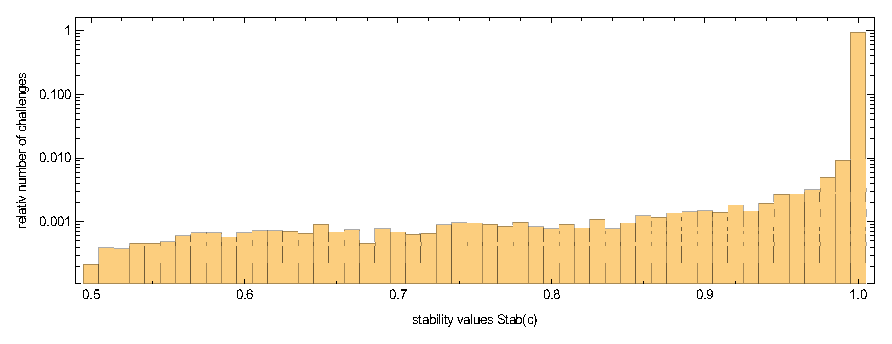
\includegraphics[width=1.00\textwidth]{images/arbiter-stability-distribution-simulation.eps}
% \noindent\includegraphics[width=1.00\textwidth, height=3cm, draft]{example-image-a}
\caption[Challenge stability distribution of an \apuf]{Challenge stability distribution of an \apuf using $32$ stages. Every challenge has been measured $100$ times. The y-axis of the graph is scaled in $log_2$ to figure the wide range of the values.} 
\label{fig:arbiterstabilitydistribution}
\end{figure}

Since \apufs can have a different number of stages it could be claimed that this has impact on the stability of the \puf.
Except for very low numbers of $\gls{n}$ Fig. \ref{fig:arbiterstabilities} displays that there is no relation and therefor no stability improvement due to the number of used stages. % paper lemma 8
In this simulation for every value of $\gls{n}$ the average of the results of $10$ independent \apufs has been build.
A challenge is here considered to be unstable if $\Stab(\gls{c}) < 95 \%$.

% Percentage of unstable challenges (Stab(c) < 0.95 %) of a random chosen set of challenges of Arbiters of different size n, avg over 10 independent instances ( 2^11 challenges)
\begin{figure}[ht]
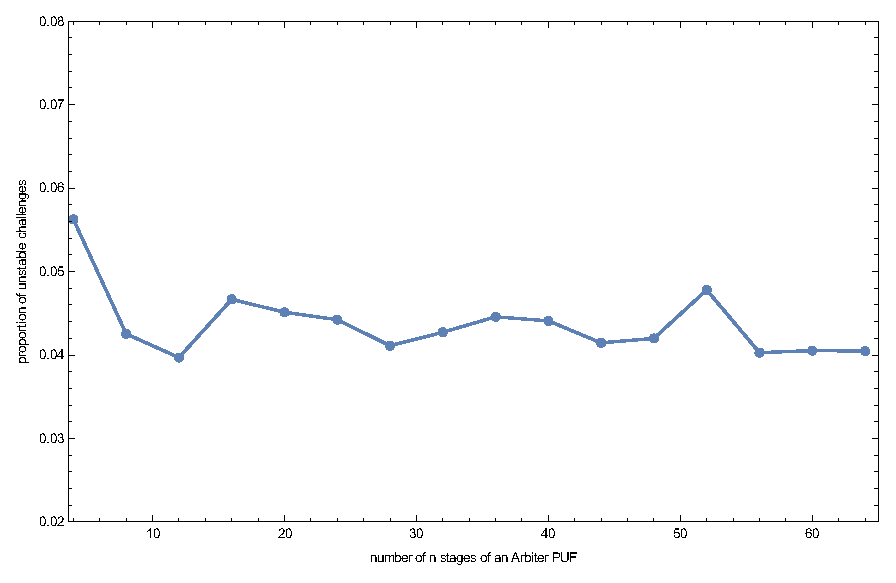
\includegraphics[width=1.00\textwidth]{images/stages-stab-simulation.eps}
% \noindent\includegraphics[width=1.00\textwidth, height=3cm, draft]{example-image-a}
\caption[Proportion of unstable challenges of an \apuf]{Proportion of unstable challenges of a random chosen set of challenges for \apufs with $\gls{n}$ stages. 
A challenges is unstable when $\Stab(\gls{c}) < 95 \%$. 
The results are the average values over $10$ individual \puf instances with the same challenge set.} 
\label{fig:arbiterstabilities}
\end{figure}

% simulation values: noise  to model ratio: ref to simulation design!
%========================================

\section{Stability Improvement by Majority Vote}
\label{sec:stabilityimprovementbymajorityvote}

To prove the stability increase achieved by \ac{MV}, Fig. \ref{fig:majorityvotestabilityimprovement} shows the decrease of unstable challenges for a growing number of votes.
The \mpuf has size $\gls{n} = 32$ and used challenges are randomly chosen.
Challenges are again considered to be unstable when $\Stab(\gls{c}) < 95 \%$.
Beside the expression of declining unstable challenges the graph has a lowering gradient which means the that the improving impact of \ac{MV} subsides with growing $\gls{m}$ as Fig. \ref{fig:majorityvotestabilityimprovementloglog} displays.
\todo{check loglogfigure!}
Hence the relative stability improvement is highest with the first increase of $\gls{m}$ as the beginning of the graph shows.
The figure shows that \ac{MV} improves the stability of an \apuf remarkable. 

% Percentage of unstable challenges (Stab(c) < 0.95 %) of a random chosen set of challenges of Arbiters of n=32 for different majority votes (2^11 challenges)
\begin{figure}[ht]
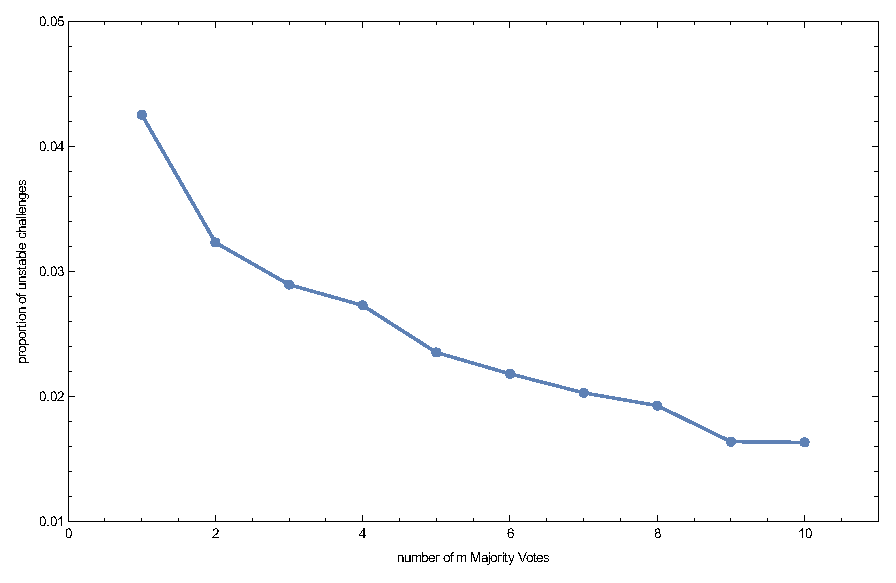
\includegraphics[width=1.00\textwidth]{images/single-votes-stab-simulation.eps}
% \noindent\includegraphics[width=1.00\textwidth, height=3cm, draft]{example-image-a}
\caption[Decrease of unstable challenges of a \mpuf]{The line graph displays the decrease of unstable challenges ($\Stab(\gls{c}) < 95 \%$) of a random chosen set of challenges for different number of $\gls{m}$ of an \mpuf.
The \mpuf has size $\gls{n} = 32$.
A decline of the stability improvement with growing $\gls{m}$ is shown by the lowering gradient of the line graph.
} 
\label{fig:majorityvotestabilityimprovement}
\end{figure}

\begin{figure}[ht]
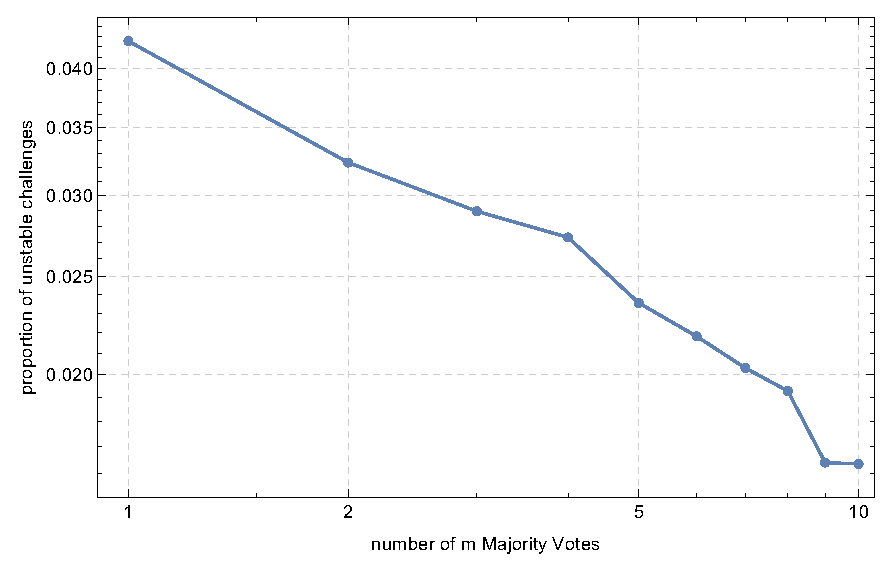
\includegraphics[width=1.00\textwidth]{images/single-votes-stab-simulation_loglog.eps}
% \noindent\includegraphics[width=1.00\textwidth, height=3cm, draft]{example-image-a}
\caption[Decreasing improvement impact by \acs{MV} of a \mpuf]{Line graph scaled in log-log to show decreasing \ac{MV} stability improving impact with growing $\gls{m}$} 
\label{fig:majorityvotestabilityimprovementloglog}
\end{figure}

%========================================

\section{Majority Vote Increase for Majority \acs{XOR} \apufs}
\label{sec:majorityvotegrowth}
% Number of needed votes for k large xor arbiter to achieve a certain stability

As only \xpufs that are large in $\gls{k}$ can not be modeled successfully by known attacks it is the purpose to be able to build arbitrary large \xpufs which have to be stable to produce a reliable output.
To achieve this with \ac{MV} the number of $\gls{m}$ votes has to be increased with a growth in $\gls{k}$ as explained in Sec. \ref{sec:majorityxorarbiter}.
Though the growth rate of $\gls{m}$ must not be too high otherwise the time to evaluate a challenge would grow to large with large \xpufs as well. %, like exponential, 
To show that this high stability can be reached using a polynomial (in $\gls{k}$) number of \acp{MV} $\gls{k}$ parallel \mpufs for different values of $\gls{k}$ are simulated.
The simulation measures the stability values of every challenge of a subset by multiple evaluations and finds the necessary number of \ac{MV} by binary search.
\todo{pseudocode}

\todo{Probability space?}

\begin{figure}[ht]
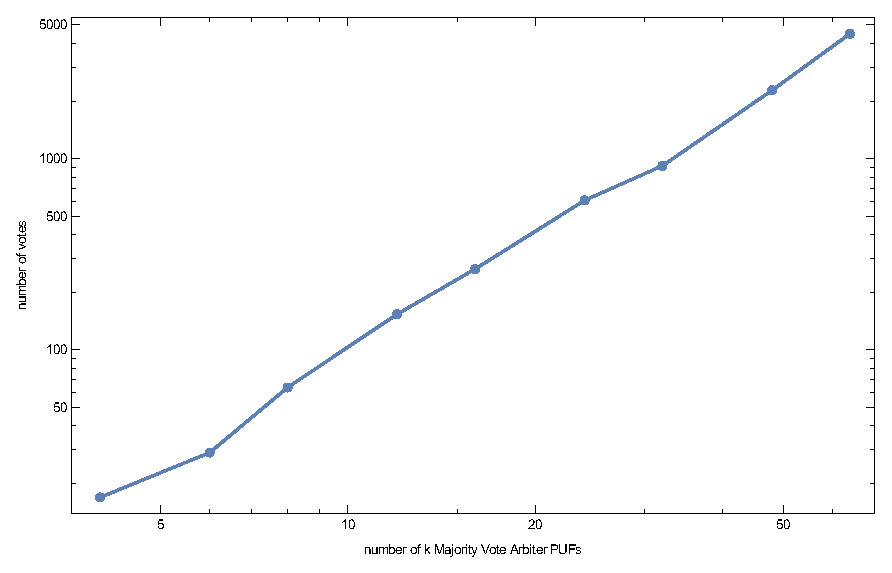
\includegraphics[width=1.00\textwidth]{images/votes-stab-simulation.eps}
% \noindent\includegraphics[width=1.00\textwidth, height=3cm, draft]{example-image-a}
\caption[Minimum number of votes need for large \mxpuf]{Minimum number of votes needed to reach $\Pr[\protect\Stab(\gls{c}) \ge 95 \%] \ge 95 \%$ for a uniformly random chosen challenge $\gls{c}$ for different numbers of $\gls{k}$ \apufs. 
The simulations uses $\gls{n} = 16$, but the results are independent of $\gls{n}$ as shown in Fig. \ref{fig:arbiterstabilities}. 
The linear graph shown in a log-log-graph confirms the polynomial growing number $\gls{m}$ of \acp{MV} of the degree $1$.
The results are the average values over $10$ individual \puf instances with independent challenge sets.} 
\label{fig:majorityvotegrowth}
\end{figure}

Fig. \ref{fig:majorityvotegrowth} shows how many votes are needed to reach a probability of $95 \%$ that a uniformly and randomly chosen challenge $\gls{c}$ has stability of at least $95 \%$, for different values of $\gls{k}$.
These are lower bounds as the \ac{XOR} operation increases the stability of a \xpuf marginal, as any even number of incorrect \apuf responses will still yield the desired output of the \xpuf. \todo{elaborate: why is this not included in your simulation? provide pseudocode to clarify.}
The polynomial increasing number of votes needed to fulfill the stability requirements for a useful PUF implementation displayed in the Figure proves that \xpufs can be build arbitrary large using \ac{MV}.

%========================================
% Figure fig:majorityvotegrowth: maybe add n=8 and n=12, so the reader can see that the results indeed do not change

\section{Stability Distribution of Large Majority \acs{XOR} \apufs}
% Stability distribution of xor arbiter

To get a more precise exposition of the stability distribution of \mxpufs size $\gls{k}$ the stability value for every challenge of a subset is simulated.
Therefore every challenge is evaluated $100$ times to compute its stability.
The example uses $32$ \mpufs with $32$ stages each.
The number of \acp{MV} needed to reach a stability of $95 \%$ with a likelihood of $95 \%$ is chosen from the results of Sec. \ref{sec:majorityvotegrowth}.
The stability distribution shown in Fig. \ref{fig:stabilitydistributionmajorityvote} was achieved by using $\gls{m} = 600$ votes
and is roughly equivalent to the distribution of an \apuf displayed in Fig. \ref{fig:arbiterstabilitydistribution}.
%and is roughly equivalent to an \apuf that has a $\sigmaNoise/\sigmaModel$ ratio that supersedes those of the basic \apuf by the order of several magnitudes.
This shows that even large \mxpufs can become stable through a feasible number of votes and even exceed stability of a basic \apuf with a larger number of \ac{MV}.

\begin{figure}[ht]
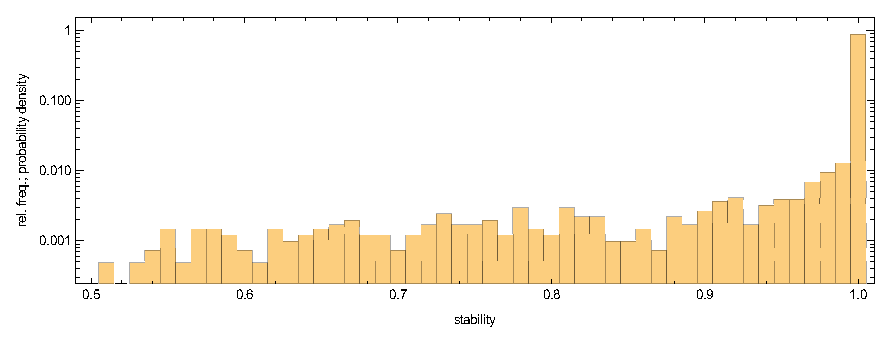
\includegraphics[width=1.00\textwidth]{images/majority-xor-stability-distribution-simulation.eps}
% \noindent\includegraphics[width=1.00\textwidth, height=3cm, draft]{example-image-a}
\caption[Challenge stability distribution of a \mxpuf]{The histogram shows the frequency of the challenge stability values of a \mxpuf with size $\gls{k} = 32$ and $32$ stages each. \ac{MV} uses $\gls{m} = 600$ to reach a stability of $95 \%$. The distribution and the amount of unstable challenges resembles the stability distribution of a \apuf as displayed in Fig. \ref{fig:arbiterstabilitydistribution}.} 
\label{fig:stabilitydistributionmajorityvote}
\end{figure}

%========================================
% fig:stabilitydistributionmajorityvote: direct comparison? it's hard to compare on different pages
% fig:stabilitydistributionmajorityvote: could the not-so-smooth histogram be caused by the effects of 'even number of errors cancel out'?











